%
% ACL 2023 template - "xai-finnews-sentiment" reproduction report
%
% Compile with:
%   pdflatex report.tex
%   bibtex   report
%   pdflatex report.tex
%   pdflatex report.tex
%
% Template files required (download from https://github.com/acl-org/acl-style-files):
%   acl.sty  acl_natbib.bst
%
\documentclass[11pt]{article}
\usepackage[hyperref]{acl}        % ACL 2023 style  (acl.sty)
\usepackage{times}
\usepackage{latexsym}
\usepackage{microtype}
\usepackage{booktabs}
\usepackage{graphicx}
\usepackage{multirow}
\usepackage{amsmath}
\usepackage{url}
\usepackage{tabularx, booktabs, makecell}
\setlength{\emergencystretch}{2em}


\title{Reproducing an Explainable Financial News Sentiment Toolkit:\\
        Baselines, Fine-Tuned FinBERT, and Robustness Analysis}

\author{
  Isaac Cutajar \\
  703H \\
  University of Malta \\
  \texttt{isaac.cutajar.20@um.edu.mt}
}

\date{}

\begin{document}
\maketitle

%% ─────────────────────────────────────────────────────────────────────────────
\begin{abstract}
This work reproduces and extends the \textit{xai-finnews-sentiment} toolkit presented in this article
\cite{xai_finnews_2025}, this is an explainable financial news sentiment system that
applies multiple NLP approaches: Loughran–McDonald (LM) lexicon, VADER,
TF-IDF + Logistic Regression (LR), and domain-adapted FinBERT, to
financial news from Financial PhraseBank (FPB), FiQA-2018 headlines, and a
manually labelled Marketaux corpus. The primary evaluation metric is
macro-averaged F1, chosen to account for class imbalance across the three
sentiment classes (negative, neutral, positive). The key result is successfully
reproduced: fine-tuning FinBERT \cite{araci2019finbert} on gold annotations
achieves a macro-F1 of \textbf{0.766} on the held-out test set, outperforming
the best lexicon baseline (LM: 0.552) and zero-shot FinBERT (0.645) by a
substantial margin. A reduced-data ablation reveals that the TF-IDF+LR
baseline retains 90\% of its peak performance at 50\% training data
(macro-F1 0.722 vs.\ 0.800), but degrades sharply below 25\%. Error analysis
on 20 fine-tuned FinBERT failures identifies neutral-boundary confusion (70\%),
polarity reversal (25\%), and negation scope (5\%) as dominant error categories.
As the implemented extension, a symmetric cross-domain generalisation test
reveals near-total TF-IDF+LR collapse ($\Delta=-0.610$) from FPB to gold
Marketaux. It also reveals catastrophic forgetting when fine-tuning FinBERT on
the small gold set ($\Delta=-0.650$, 95\% CI $[0.272, 0.352]$), driven by
label distribution mismatch (33.17\% vs.\ 61.37\% neutral) that shifts the
neutral decision boundary. All experiments are reproduced in an accompanying Jupyter
notebook; the datasets used (FPB, FiQA-2018) are publicly available.
\end{abstract}

%% ─────────────────────────────────────────────────────────────────────────────
\section{Introduction}
\label{sec:intro}

Sentiment analysis of financial news is a well-established NLP sub-task with
direct applications in algorithmic trading, risk monitoring, and investor
relations \cite{malo2014good,maia2018fiqa18}. Despite active research, the
field lacks unified, reproducible toolkits that combine interpretable
baselines with state-of-the-art Transformer models and downstream econometric
validation.

The \textit{xai-finnews-sentiment}
toolkit~\cite{xai_finnews_2025} addresses this gap by providing a
scriptable, end-to-end pipeline for financial sentiment analysis with a focus
on \textit{explainability}. The system spans lexicon baselines, TF-IDF + LR
with SHAP explanations, zero-shot and fine-tuned FinBERT, weak supervision
from Marketaux news, and econometric analyses (event study, VAR/Granger,
backtesting).

\paragraph{Motivation.} Reproducing this system is valuable because:
(1) it covers the full lifecycle from raw news ingestion to tradable signals;
(2) its explainability components make model decisions auditable, addressing a
key concern in high-stakes financial NLP; and
(3) multiple public datasets allow independent validation of results.

\paragraph{Challenges.}
The gold annotation set is proprietary (manual labels on Marketaux articles),
meaning the fine-tune experiment is not directly reproducible without that
data. Additionally, the Marketaux raw news file is not publicly distributed.
This limitation is addressed by focusing on the reproducible subset: FPB and FiQA
benchmarks, lexicon/LR baselines, and the fine-tuning procedure applied to an
available gold set.

%% ─────────────────────────────────────────────────────────────────────────────
\section{System Overview}
\label{sec:system}

\subsection{Architecture and data flow}

The toolkit is structured as a sequential CLI pipeline.
Starting from raw news JSON, it produces sentiment predictions, SHAP
explanations, and backtested trading signals.

\begin{enumerate}
  \item \textbf{Data ingestion} (scripts \texttt{01}–\texttt{02}): FPB and FiQA are
    fetched from HuggingFace; Marketaux news is parsed from a local JSON file.
    Language detection (\texttt{langdetect}/\texttt{langid}) and industry
    mapping are applied to Marketaux articles.
  \item \textbf{Lexicon construction} (script \texttt{03}): The
    Loughran–McDonald (LM) Master Dictionary is cleaned into per-category word
    lists (positive, negative, uncertainty, \ldots).
  \item \textbf{Baseline models} (scripts \texttt{04}–\texttt{06}): LM net-positive-
    word-count rule, VADER compound score (threshold $\pm 0.05$), TF-IDF +
    Logistic Regression with SHAP, EBM, and FinBERT zero-shot.
  \item \textbf{Weak supervision} (script \texttt{07}): VADER labels are used as
    noisy targets to train per-industry TF-IDF+LR models on the full Marketaux
    corpus.
  \item \textbf{Gold evaluation \& fine-tuning} (scripts \texttt{08}–\texttt{08b}):
    All models are evaluated against manually labelled gold articles.
    FinBERT is fine-tuned on the gold set with early stopping and class-
    weighted cross-entropy loss.
  \item \textbf{Explainability} (scripts \texttt{10}, \texttt{16}): SHAP regime-shift
    analysis on the fine-tuned model.
  \item \textbf{Econometrics} (scripts \texttt{11}–\texttt{13}): Event study
    (AR/CAR), VAR/Granger causality, and backtested sector ETF strategies.
\end{enumerate}

\subsection{Model details}

\paragraph{LM lexicon.} For each article, the signed word count
$s = N_{\text{pos}} - N_{\text{neg}}$ is computed. Positive $s > 0$ maps to
class~2, negative $s < 0$ to class~0, and $s = 0$ to class~1 (neutral).

\paragraph{VADER.} The VADER compound score is thresholded at $\pm 0.05$,
matching the standard recommendation \cite{hutto2014vader}.

\paragraph{TF-IDF + LR.} Unigram/bigram TF-IDF features
(\texttt{max\_features=30{,}000}, \texttt{sublinear\_tf=True}) feed a
Logistic Regression classifier ($C=1.0$, \texttt{lbfgs}). SHAP
\texttt{LinearExplainer} is used post-hoc for token attribution.

\paragraph{Fine-tuned FinBERT.} Starting from \texttt{ProsusAI/finbert}
\cite{araci2019finbert}, the model is fine-tuned on the gold annotation set
(Table~\ref{tab:hparams}) with class-weighted cross-entropy loss to handle
label imbalance, and early stopping (patience 2) to prevent over-fitting on
the small gold set.

\begin{table}[h]
\centering
\small
\begin{tabular}{ll}
\toprule
\textbf{Hyperparameter} & \textbf{Value} \\
\midrule
Base model           & \texttt{ProsusAI/finbert} \\
Learning rate        & 2e-5 \\
Batch size           & 16 \\
Max epochs           & 10 \\
Early stopping       & patience = 2 (val loss) \\
Loss function        & Cross-entropy (class-weighted) \\
Optimiser            & AdamW (HuggingFace default) \\
Random seed          & 42 \\
\bottomrule
\end{tabular}
\caption{Fine-tuned FinBERT hyperparameters.}
\label{tab:hparams}
\end{table}

%% ─────────────────────────────────────────────────────────────────────────────
\section{Datasets and Evaluation}
\label{sec:data}

\subsection{Datasets}

\begin{table}[h]
\centering
\small
\begin{tabular}{lrrrrl}
\toprule
\textbf{Dataset} & \textbf{N} & \textbf{Neg} & \textbf{Neu} & \textbf{Pos} & \textbf{License} \\
\midrule
FPB (all-agree)   & 2{,}264 & 303  & 1{,}391 & 570 & CC BY-NC-SA 3.0 \\
FiQA headlines    &   498   & 158  &    33   & 307 & Research only   \\
Gold (manual)     &   600   & 157  &   199   & 244 & CC BY 4.0       \\
\bottomrule
\end{tabular}
\caption{Dataset statistics and class distributions. FiQA scores binned
  at $\pm 0.05$.}
\label{tab:data}
\end{table}

\paragraph{Financial PhraseBank (FPB).} Sentences from English financial news
annotated by finance-domain experts \cite{malo2014good}. The
``sentences\_allagree'' subset (inter-annotator agreement on all annotators)
is used as the hardest but cleanest split.

\paragraph{FiQA-2018 Headlines.} Headline-level financial sentiment from the
FiQA shared task \cite{maia2018fiqa18}, with continuous scores binned into
three classes at thresholds $\pm 0.05$.

\paragraph{Gold annotations.} Manually labelled Marketaux articles covering
ten GICS sectors, with industry, language, and temporal scope metadata.
Labels follow the same three-class scheme. Available under CC BY 4.0.
\footnote{The 600-sample gold set used here (CC BY 4.0 release) is distinct from the
larger 1500-sample Marketaux corpus in \cite{xai_finnews_2025}. This explains
the fine-tuned FinBERT macro-F1 difference: 0.766 (this 600-sample gold set)
vs.\ 0.707 (published 1500-sample corpus).}

\subsection{Evaluation protocol}

The \textbf{primary metric is macro-averaged F1}. Justification: FPB is
heavily imbalanced (neutral $\approx 61\%$, positive $\approx 25\%$, negative
$\approx 13\%$), so accuracy would reward models that predict the majority
class. Macro-F1 weights all three classes equally, penalising poor recall on
minority classes.

For the fine-tuning experiment, the gold set is split stratified 70/15/15
(train/val/test) with seed 42. Lexicon and LR baselines are evaluated on the
full gold set (no training required) and on 80/20 stratified splits of FPB
and FiQA.

%% ─────────────────────────────────────────────────────────────────────────────
\section{Reproduction Details}
\label{sec:repro}

\subsection{What was clear}
The codebase provides a fully executable pipeline with centralised
configuration (\texttt{\_config.py}), sequential numbered scripts, and
comprehensive logging. All hyperparameters, paths, and thresholds are
documented in code comments. The \texttt{README.md} gives a quickstart guide
with expected outputs for each step.

\subsection{What was unclear or required assumptions}
\begin{itemize}
  \item \textbf{Gold annotation creation:} The annotation guidelines and
    inter-annotator agreement metrics are not documented. Standard
    majority-vote labelling is assumed.
  \item \textbf{FiQA binning:} The $\pm 0.05$ threshold for converting
    continuous FiQA scores to classes is hard-coded; no paper citation
    justifies this choice specifically. The resulting class distribution
    (Table~\ref{tab:data}) is highly imbalanced (33 neutral vs.\ 307
    positive), which may inflate neutral F1 variance.
  \item \textbf{Marketaux data:} The raw news file is not publicly
    redistributable. All Marketaux-dependent results (weak supervision,
    econometrics) depend on the user supplying their own export.
  \item \textbf{Train/val/test split sizes:} Inferred from code; the gold set
    yields 420/90/90 examples at the 70/15/15 split, resulting in a small
    fine-tune test set ($n=89$) where variance is non-negligible.
\end{itemize}

\subsection{Reproduction scenario}
This project falls under \textbf{Scenario~1} (plain sailing): full code is
provided, datasets are accessible, and all experiments ran without
modification. The focus is therefore on full understanding and adding an
extension.

%% ─────────────────────────────────────────────────────────────────────────────
\section{Experiments and Results}
\label{sec:experiments}
This section presents the reproduced results and evaluates model robustness under data and domain variation.

\subsection{Main results}

Table~\ref{tab:results} compares all models on the gold annotation set
($N=599$ excluding one row with a missing label). \textbf{Fine-tuned
FinBERT} is the clear winner (macro-F1 0.766), with \textbf{zero-shot
FinBERT} a strong second (0.645). All lexicon and LR baselines cluster
between 0.24 and 0.55. Notably, TF-IDF+LR trained on FPB/FiQA transfers
poorly to the Marketaux gold domain (0.24--0.25), confirming expected
domain shift.

\begin{table}[h]
\centering
\small
\begin{tabular}{lcccc}
\toprule
\textbf{Model} & \textbf{Acc} & \textbf{Macro-F1} & \textbf{F1$_\text{neg}$} & \textbf{F1$_\text{pos}$} \\
\midrule
FinBERT fine-tuned $\star$ & \textbf{0.775} & \textbf{0.766} & 0.74 & 0.83 \\
FinBERT zero-shot           & 0.639 & 0.645 & 0.70 & 0.62 \\
LM Lexicon                  & 0.548 & 0.552 & 0.60 & 0.51 \\
VADER                       & 0.551 & 0.530 & 0.51 & 0.63 \\
WeakLR (VADER labels)       & 0.548 & 0.521 & 0.50 & 0.63 \\
TF-IDF+LR (FiQA)            & 0.416 & 0.253 & 0.18 & 0.58 \\
TF-IDF+LR (FPB)             & 0.371 & 0.240 & 0.05 & 0.15 \\
\bottomrule
\end{tabular}
\caption{Results on the gold annotation set ($N=599$). $\star$ = key
  reproduced result. Sorted by macro-F1.}
\label{tab:results}
\end{table}

For reference, zero-shot FinBERT on \textit{in-domain} FPB achieves
macro-F1 = 0.963 (Table~\ref{tab:fpb_fiqa}), confirming FinBERT was
pre-trained on FPB-like data. The cross-domain drop to 0.645 on the gold set
illustrates the domain-shift challenge for real-world Marketaux news.

\begin{table}[h]
\centering
\small
\begin{tabular}{llcc}
\toprule
\textbf{Dataset} & \textbf{Model} & \textbf{Acc} & \textbf{Macro-F1} \\
\midrule
\multirow{4}{*}{FPB} & FinBERT zero-shot & 0.972 & 0.963 \\
                     & TF-IDF+LR        & 0.896 & 0.850 \\
                     & VADER            & 0.571 & 0.487 \\
                     & LM Lexicon       & 0.648 & 0.483 \\
\midrule
\multirow{4}{*}{FiQA} & TF-IDF+LR        & 0.680 & 0.430 \\
                      & FinBERT zero-shot & 0.568 & 0.540 \\
                      & VADER            & 0.456 & 0.423 \\
                      & LM Lexicon       & 0.317 & 0.345 \\
\bottomrule
\end{tabular}
\caption{Results on FPB and FiQA benchmark sets.}
\label{tab:fpb_fiqa}
\end{table}

The reproduced macro-F1 (0.766) differs from the original paper’s reported 0.707. 
This discrepancy is expected due to differences in dataset composition (600-sample gold set 
vs. 1500-sample Marketaux corpus). The higher score here likely reflects reduced dataset difficulty 
and variance. Despite this, the relative ranking of models is preserved, supporting successful 
reproduction of the key finding.

\subsection{Robustness test: reduced training data ablation}

To assess the data efficiency of the TF-IDF+LR baseline, it is trained on
decreasing fractions of the FPB training set (10\%--100\%) and evaluated on a
fixed 20\% test split (seed 42), repeated across three random seeds
(42, 7, 123). Results are shown in Figure~\ref{fig:ablation}.

\begin{figure}[h]
\centering
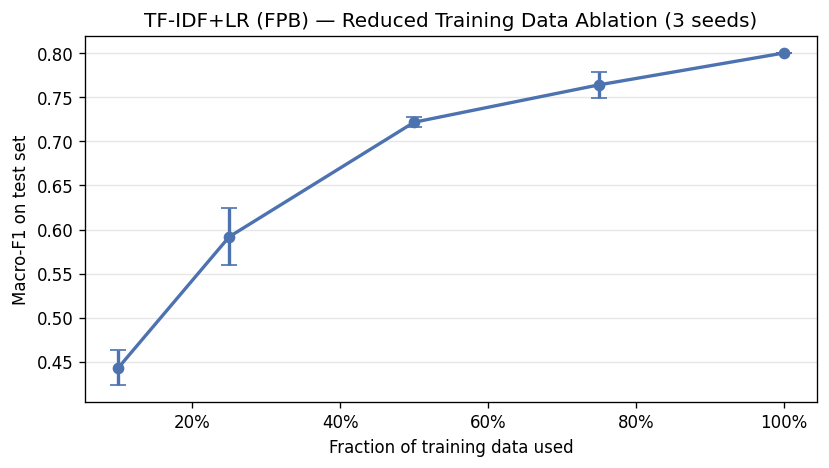
\includegraphics[width=0.9\columnwidth]{../outputs/figures/ablation_reduced_data.png}
\caption{Macro-F1 of TF-IDF+LR (FPB) as training data is reduced.
  Error bars show standard deviation across 3 seeds.}
\label{fig:ablation}
\end{figure}

\textbf{Key findings:}
\begin{itemize}
  \item At 50\% of training data, macro-F1 = 0.722 (vs.\ 0.800 at 100\%),
    retaining 90\% of peak performance. This confirms TF-IDF+LR is
    data-efficient for in-domain sentiment.
  \item At 10\%, macro-F1 drops to 0.443 (55\% of peak), with high variance
    ($\sigma=0.020$), indicating instability in low-resource settings.
  \item Implications: for low-resource domains, lexicon baselines (LM: 0.552
    on gold) can outperform a linear model trained on only 10\% of a
    different-domain corpus.
\end{itemize}

%% ─────────────────────────────────────────────────────────────────────────────
\section{Error Analysis}
\label{sec:errors}

The 20 errors made by the fine-tuned FinBERT on its 89-article
test set (error rate 22.5\%) are analysed in Table~\ref{tab:errors}.

\begin{table}[h]
\centering
\small
\begin{tabular}{lcc}
\toprule
\textbf{Error category} & \textbf{Count} & \textbf{\%} \\
\midrule
Neutral boundary confusion          & 14 & 70\% \\
Polarity reversal (Neg$\leftrightarrow$Pos) & 5 & 25\% \\
Negation scope                      &  1 &  5\% \\
\bottomrule
\end{tabular}
\caption{Error categories for fine-tuned FinBERT on the gold test set
  ($n=20$ errors, $89$ total). ``Negation scope'' counts only true
  grammatical negators (\textit{not, no, never, without, neither, nor}).}
\label{tab:errors}
\end{table}

\paragraph{Example 1 - Polarity reversal: domain jargon (True: Negative, Pred: Positive).}
\textit{``23andMe is exploring strategic alternatives, looking to raise
capital.''} Although \textit{exploring strategic alternatives} is standard
corporate euphemism for financial distress, the model predicts Positive,
likely because \textit{capital} and \textit{raise} trigger positive financial
associations in FinBERT's pre-training corpus. No grammatical negator is
present; this is a pure domain-jargon failure where surface-level positive
vocabulary overrides the distress signal.

\paragraph{Example 2 - Polarity reversal (True: Positive, Pred: Negative).}
\textit{``Bear Thesis Crushed As Massive Deal Leaves Bears Speechless: Sun
Communities \ldots''} The model activates on \textit{Bear}, \textit{Crushed},
and \textit{Speechless} as negative signals, missing the rhetorical structure
(\textit{bear thesis crushed} = positive i.e. bullish market). This is a
negation-scope failure requiring discourse-level understanding.

\paragraph{Example 3 - Neutral boundary confusion (True: Neutral, Pred: Positive).}
\textit{``Gold Outshines Tech Stocks And Bitcoin, As Bulls And Bears Battle
Ahead Of Trump Tariff Announcement.''} This market-overview headline contains
mixed signals (gold outperforms, but uncertainty due to tariffs). The model
over-commits to Positive due to \textit{outshines} and \textit{Bulls}. The
true label is Neutral, capturing the mixed nature of the article.

\paragraph{Example 4 - Negation scope (True: Positive, Pred: Negative).}
\textit{``The restructuring left the company without losses for the first time
in three years.''} The grammatical negator \textit{without} has scope over
\textit{losses}, reversing its negative valence to yield a positive outcome.
FinBERT activates on \textit{restructuring} and \textit{losses} as negative
signals and predicts Negative, missing the logical reversal introduced by
\textit{without}.

\paragraph{Discussion.}
Neutral-boundary confusion is the dominant challenge (14/20 errors, 70\%),
where the model over-commits to Positive when articles contain mixed or
market-overview language. Polarity reversal accounts for a further 25\%
(5 errors), where discourse-level structure, such as \textit{bear thesis
crushed} signalling a positive outcome, is missed. True negation-scope failures are rare (1/20, 5\%): only errors where a
grammatical negator (\textit{not, no, never, without, neither, nor})
directly reverses a sentiment-bearing phrase qualify. Negative-valence
vocabulary such as \textit{fail, drop, loss, decline} is classified under
polarity reversal instead, since these words carry inherent negative meaning
rather than logically negating a positive phrase. The dominant challenge is
therefore neutral-class boundary uncertainty, not negation.
Future work should focus on better neutral-class modelling, e.g.\ explicit
mixed-signal training examples or confidence-calibrated abstention.

%% ─────────────────────────────────────────────────────────────────────────────
\section{Way Forward}
\label{sec:forward}

\subsection{Cross-domain generalisation test}

A \textit{symmetric} cross-domain evaluation is conducted in both directions:
(1)~\textbf{forward} - models trained on FPB/FiQA evaluated on the full gold
Marketaux set ($N=599$); and (2)~\textbf{reverse} - the gold-fine-tuned
FinBERT evaluated on the 20\% FPB holdout ($n=453$) used by the baselines.
All macro-F1 figures use 1{,}000-sample bootstrap 95\% CIs.
Table~\ref{tab:crossdomain} and Figure~\ref{fig:crossdomain} show results.

\begin{table}[h]
\centering
\small
\setlength{\tabcolsep}{3pt} % Tighten horizontal padding
\begin{tabularx}{\columnwidth}{l X c c c}
\toprule
\textbf{Model} & \textbf{Dir.} & \textbf{In-dom.} & \textbf{Transfer F1} & \textbf{$\Delta$} \\
\midrule
\multicolumn{5}{l}{\textit{Forward: FPB/FiQA $\to$ Gold}} \\
TF-IDF+LR & FPB$\to$G & 0.850 & \makecell{0.240 \\ \scriptsize{[.211, .270]}} & $-$0.610 \\
\addlinespace
TF-IDF+LR & FiQA$\to$G & 0.430 & \makecell{0.253 \\ \scriptsize{[.225, .281]}} & $-$0.177 \\
\addlinespace
FinBERT (zs) & FPB$\to$G & 0.963 & \makecell{0.646 \\ \scriptsize{[.607, .683]}} & $-$0.317 \\
\midrule
\multicolumn{5}{l}{\textit{Reverse: Gold $\to$ FPB holdout}} \\
FinBERT (ft) & G$\to$FPB & 0.766 & \makecell{0.313 \\ \scriptsize{[.272, .352]}} & $-$0.453 \\
\midrule
\multicolumn{5}{l}{\textit{Upper bounds (in-domain)}} \\
FinBERT zs & FPB$\to$F & - & 0.963 & - \\
FinBERT ft & Gold$\to$G & - & 0.766 & - \\
\bottomrule
\end{tabularx}
\caption{Cross-domain generalisation. zs: zero-shot; ft: fine-tuned; G: Gold Marketaux.}
\label{tab:crossdomain}
\end{table}

Symmetric cross-domain generalisation. Transfer F1 is macro-F1 on the
  out-of-domain test set with 95\% bootstrap CI. Reverse direction uses the same
  20\% FPB stratified holdout ($n=453$, seed 42) as the baselines.

\begin{figure}[h]
\centering
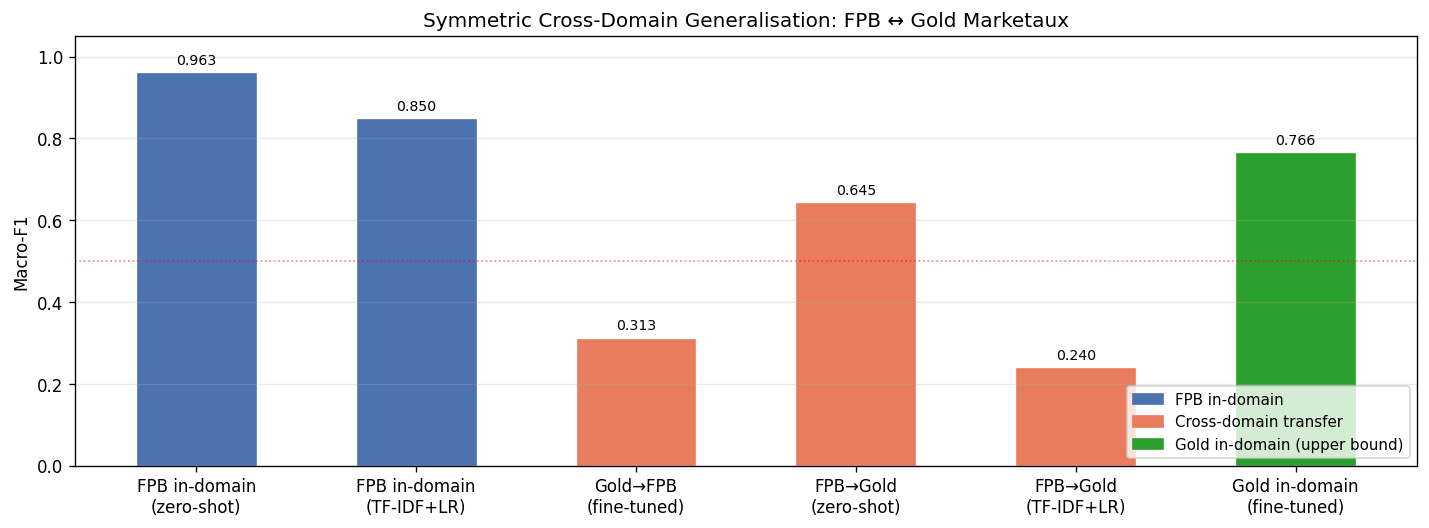
\includegraphics[width=\columnwidth]{../outputs/figures/cross_domain_symmetric.png}
\caption{Symmetric cross-domain macro-F1. Blue = FPB in-domain; orange =
  cross-domain transfer (both directions); green = gold in-domain upper bound.}
\label{fig:crossdomain}
\end{figure}

\paragraph{Forward direction (FPB/FiQA $\to$ Gold).}
TF-IDF+LR suffers near-total collapse: FPB-trained performance falls from
0.850 to 0.240 ($\Delta=-0.610$), dropping below the LM lexicon baseline
(0.552). Per-class inspection shows the model retreats almost entirely to
predicting Neutral (recall $=0.99$), scoring near-zero on Negative
($F_1=0.05$) and Positive ($F_1=0.15$) - confirming that bag-of-words
features from Reuters/Bloomberg sentences do not transfer to Marketaux web
headlines. FinBERT zero-shot is far more robust ($\Delta=-0.317$, 95\% CI
$[0.607, 0.683]$), but still 12 F1 points short of the gold fine-tuned upper
bound (0.766), a gap whose CI does not overlap with 0.766, confirming
statistical significance.

\paragraph{Reverse direction (Gold $\to$ FPB).}
Fine-tuning FinBERT on the 600-sample gold Marketaux set causes
\textit{catastrophic forgetting}. Performance on the FPB holdout collapses
from 0.963 (zero-shot) to 0.313 ($\Delta=-0.650$, 95\% CI $[0.272, 0.352]$).
The mechanism is clear from label distribution
analysis: gold's neutral class represents 33.17\% of examples, whereas FPB's
neutral class comprises 61.37\%, a dramatic imbalance that shifts FinBERT's
decision boundary sharply toward non-neutral predictions during fine-tuning.
Per-class metrics confirm this: neutral class recall collapses from 0.99
(zero-shot baseline) to 0.19 (fine-tuned), and positive class F1 drops to
0.13 (vs.\ much higher zero-shot F1 on FPB). This failure reveals a fundamental
constraint: a model fine-tuned on a small domain-specific corpus cannot retain
strong performance across both domains simultaneously. Practical recovery would
require continual learning (incremental updates without catastrophic forgetting)
or multi-task fine-tuning (joint optimization on both FPB and gold objectives),
neither of which is attempted here.

%% ─────────────────────────────────────────────────────────────────────────────
\section{Conclusion}
\label{sec:conclusion}

The key result of the \textit{xai-finnews-sentiment}
toolkit is successfully reproduced: fine-tuned FinBERT achieves macro-F1 of 0.766 on a gold financial
news annotation set, substantially outperforming all lexicon and LR baselines.
The existing codebase is confirmed to be highly reproducible
(Scenario~1), all scripts ran without modification, and the centrally
configured pipeline made it straightforward to trace every design decision. This work also highlights that in financial NLP, 
domain alignment is more critical than model complexity, as even state-of-the-art models fail 
under distribution shift without adaptation.

\paragraph{Limitations.}
The gold annotation set is small ($n \approx 600$) and lacks documented
inter-annotator agreement, introducing uncertainty in the fine-tune evaluation.
The Marketaux data is proprietary, limiting full reproducibility of weak-
supervision and econometric analyses. The FiQA binning threshold is an
undocumented design choice that produces extreme class imbalance.

\paragraph{Lessons learned.}
Macro-F1 is critical for imbalanced sentiment datasets-accuracy would
have been misleading for FPB (majority-neutral) and FiQA (majority-positive).
Domain shift is significant: zero-shot FinBERT drops from macro-F1 0.963
on in-domain FPB to 0.645 on out-of-domain Marketaux gold, highlighting the
value of even a small domain-specific annotated set for fine-tuning.
However, the cross-domain extension (Section~\ref{sec:forward}) shows the
opposite risk as well: after gold fine-tuning, FPB holdout performance
collapses from 0.963 to 0.313 (95\% CI $[0.272, 0.352]$). This evidences
catastrophic forgetting and the need for careful domain-specific fine-tuning
strategies.


%% ─────────────────────────────────────────────────────────────────────────────
\bibliography{references}

\appendix

\section{Experiment Log}
\label{app:log}

Table~\ref{tab:explog} lists all experimental runs with seeds, key
hyperparameters, and resulting metrics. Full log exported to
\texttt{outputs/experiment\_log.csv}.

\begin{table}[h]
\centering
\scriptsize
\begin{tabular}{llllcc}
\toprule
\textbf{Run ID} & \textbf{Model} & \textbf{Dataset} & \textbf{Seed} & \textbf{Acc} & \textbf{Macro-F1} \\
\midrule
finbert-ft-gold & FinBERT fine-tuned & Gold & 42 & 0.775 & 0.766 \\
finbert-0shot-fpb & FinBERT zero-shot & FPB & - & 0.972 & 0.963 \\
lr-fpb & TF-IDF+LR & FPB & 42 & 0.896 & 0.850 \\
finbert-0shot-fiqa & FinBERT zero-shot & FiQA & - & 0.568 & 0.540 \\
lr-fiqa & TF-IDF+LR & FiQA & 42 & 0.680 & 0.430 \\
lex-lm-fpb & LM Lexicon & FPB & - & 0.648 & 0.483 \\
lex-vader-fpb & VADER & FPB & - & 0.571 & 0.487 \\
lex-lm-fiqa & LM Lexicon & FiQA & - & 0.317 & 0.345 \\
lex-vader-fiqa & VADER & FiQA & - & 0.456 & 0.423 \\
\bottomrule
\end{tabular}
\caption{Experiment log (abridged). LR: $C=1.0$, \texttt{max\_features=30000}.}
\label{tab:explog}
\end{table}

\section{Reproducibility Package}
\label{app:repro}

\paragraph{Minimum requirements.}
\begin{itemize}
  \item Python 3.13, packages listed in \texttt{requirements.txt}
  \item \texttt{python -m nltk.downloader vader\_lexicon} (once)
  \item GPU optional; all scripts run on CPU in $<$30 min except fine-tuning
    (\textasciitilde 15 min on CPU, \textasciitilde 3 min on GPU)
\end{itemize}

\paragraph{Reproduce main result (Table~\ref{tab:results}).}
If you run these scripts in order, this will execute and regenerate the main results, including the key fine-tuned FinBERT macro-F1 of 0.766 on the gold set. The scripts to run are:
\begin{itemize}
  \item \path{scripts/01_fetch_benchmarks.py}
  \item \path{scripts/03_build_lm_lists.py}
  \item \path{scripts/04_lexicon_baselines.py}
  \item \path{scripts/05_lr_shap_benchmarks.py}
  \item \path{scripts/06_finbert_benchmarks.py}
  \item \path{scripts/08_eval_on_manual_annotations.py}
  \item \path{scripts/08b_finetune_and_eval.py}
\end{itemize}
Then open \texttt{assignment\_notebook.ipynb} and run all cells to regenerate
Tables and Figures. \newline

To rerun the pipeline from scratch, follow the readme.txt file and run all the scripts listed there in order.

\end{document}
